\section{Modelado de formas con conjuntos difusos}

Los descriptores relativos a formas hasta la fecha definen propiedades matemáticas de la misma, pero no tratan de definirla usando conceptos. La curvatura, uno de los descriptores más utilizados es buena muestra de ello. Pese a ser un concepto matemático común, no nos aporta ningún tipo de información, solo un conjunto de valores que la representa. Utilizando la lógica difusa, se puede tratar de modelar conceptos lingüísticos comunes en el habla, tales como si un objeto es alargado o redondeado, adaptándose a las posibles imprecisiones del mundo real.\\

Este desarrollo propio, tiene el objetivo final de poder modelar formas complejas utilizando la lógica difusa. Se encuentra enmarcado dentro de la Beca de Iniciación a la Investigación desarrollada también junto al director de este trabajo, partiendo desde cero para intentar modelar completamente las formas. En una primera incursión en este tema\cite{JChamorro}, se trata de definir los conceptos más básicos sobre contornos, la ``linealidad'', la ``curvacidad'' y la ``verticidad'', que servirán de base para futuras propiedades. En este trabajo se muestran la definición de dichos conceptos, además de algunas correcciones y mejoras aportadas al artículo original.\\

\subsection{Linealidad}

\subsubsection{Definición}
La linealidad define en que grado un segmento del contorno es una línea.\\

Sea $ C = \left\lbrace p_i = \left( x_i,y_i\right) \right\rbrace_{0\leq i\leq n}$ un contorno definido como un conjunto ordenado cíclico. Sea $S^C_{ij} = \left\lbrace p_k \in C \right\rbrace_{i \leq k \leq j}$ y $\Theta^C = \left\lbrace S^C_{ij}\right\rbrace_{i \neq j}$.\\

Definimos la linealidad a través de un conjunto difuso:\\

\[
\ \tilde{L}:\Theta^C \rightarrow \left[ 0,1 \right]
\]

Cuya función de pertenencia es:\\

\[
\ \tilde{L} \left(S^C_{ij}\right) = A \left( 1-\frac{\sum^j_{k=i} \parallel p_k - \widehat{p}_k \parallel}{\sum^j_{k=i} \parallel p_k - \overline{p}_{S^C_{ij}} \parallel} \right)
\]

Donde $\parallel p_k - \widehat{p}_k \parallel$ es la distancia entre el punto $p^k$ y la recta de regresión de los puntos del segmento, $\parallel p_k - \overline{p}_{S^C_{ij}} \parallel$ es la distancia entre el punto $p^k$ y la media de los puntos del segmento $\overline{p}_{S^C_{ij}}$ y $A$ es una función de ajuste.\\

Dado que los puntos $\widehat{p}_k$ son obtenidos a través de la proyección a una recta de regresión, el numerador de la fórmula será siempre menor o igual que el denominador. Obtenemos por tanto un valor entre 0 y 1, valiendo 0 si el ajuste de la recta de regresión es perfecto ---es decir, el segmento es una recta perfecta--- y 1 en el peor de los casos. Restando este valor a 1, obtenemos lo que buscábamos, un indicador que nos devuelva 1 si estamos ante una recta y vaya bajando hasta el 0, según los puntos del contorno se vayan alejando de una recta.\\

Sin embargo, el rango obtenido al aplicarlo a imágenes reales no varía en todo el intervalo $\left[ 0,1 \right]$, lo que hace necesaria la introducción de la función de ajuste $A$. Para la selección de dicha función, se diseñó un experimento en el que se transformaba una línea recta en una semicircunferencia. La fórmula para la creación de estos segmentos intermedios es:\\

\[
\ y = (1-p)+ p \sqrt{1-x^2}
\]

Donde $p$ es el porcentaje de semicircunferencia de la forma. En la figura \ref{fig2} podemos encontrar los resultados de calcular la linealidad sin ningún tipo de ajuste, con 100 pasos intermedios.\\

\begin{figure}[H]
\begin{center}

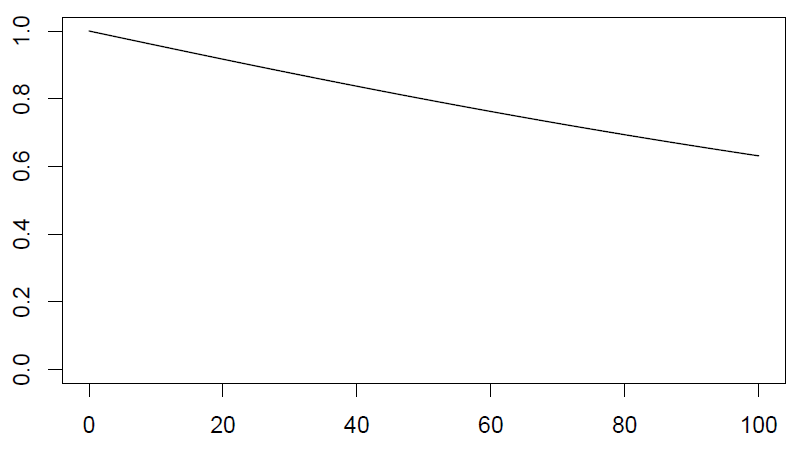
\includegraphics[width=0.9\textwidth]{img/linea-curva.png}
\end{center}

\caption{Linealidad sin ajuste.}
\label{fig2}
\end{figure}

Una primera aproximación fue pensar en funciones de ajuste del tipo $A(x) = x^q$ con $q \in \mathcal{R}^+$. Pero como podemos ver en la figura \ref{fig3}, necesitamos un $q$ grande para llevar los valores a un valor cercano a 0, lo que deforma la gráfica.\\

\begin{figure}[H]
\begin{center}

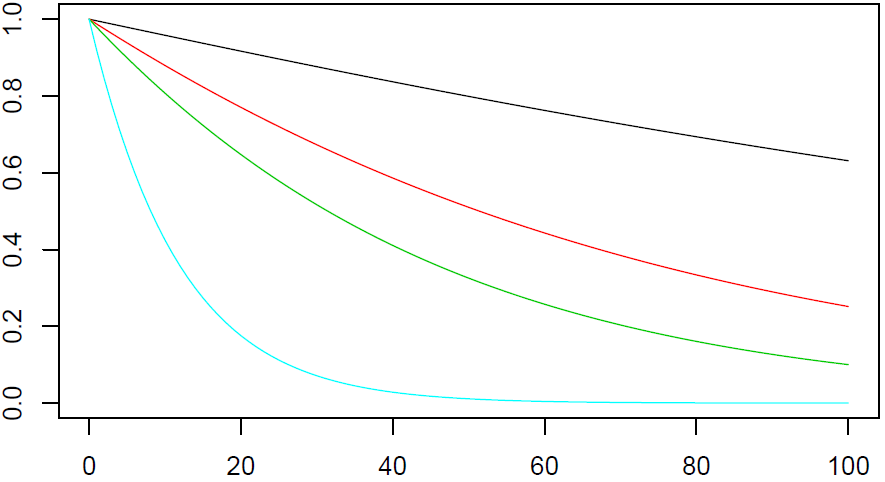
\includegraphics[width=0.9\textwidth]{img/Ajuste-q.png}
\end{center}

\caption{Linealidad con ajuste tipo potencias. q = 3,5,20.}
\label{fig3}
\end{figure}

Por tanto, se pasó a un ajuste de tipo "cambio de rango". Tomamos como posibles A la familia de funciones:\\

\[
\ A(x,\alpha) = \texttt{max}\left(\frac{x-\alpha}{1-\alpha} ,0\right)
\]

Queda libre el ajuste de $\alpha$. Este valor está asociado al ángulo del arco de circunferencia que consideramos que ya no es una línea. En la figura \ref{fig4} tenemos una gráfica que relaciona el ángulo del arco de circunferencia con su valor de $\alpha$.\\

\begin{figure}[H]
\begin{center}

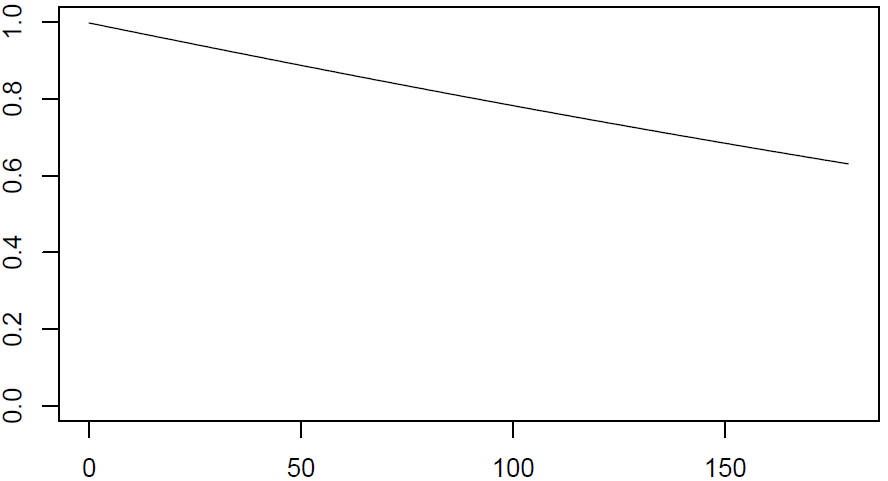
\includegraphics[width=0.9\textwidth]{img/experimento-angulo.png}
\end{center}

\caption{Linealidad de los arcos de circunferencia.}
\label{fig4}
\end{figure}

Podemos aproximar la línea de la figura \ref{fig4} para obtener una relación rápida entre el arco de circunferencia que consideramos que ya no es una linea y el $\alpha$ que debemos fijar. Obtenemos la siguiente función:\\

\[
\ \alpha(\Theta) = 1- \frac{0.37}{\pi} \Theta
\]

Utilizando $\alpha = 0.63$ en el experimento de la figura \ref{fig2}, obtenemos el ajuste de la figura \ref{fig5}, que se comporta de manera lineal y que cubre de manera efectiva el rango [0,1].\\


\begin{figure}[H]
\begin{center}

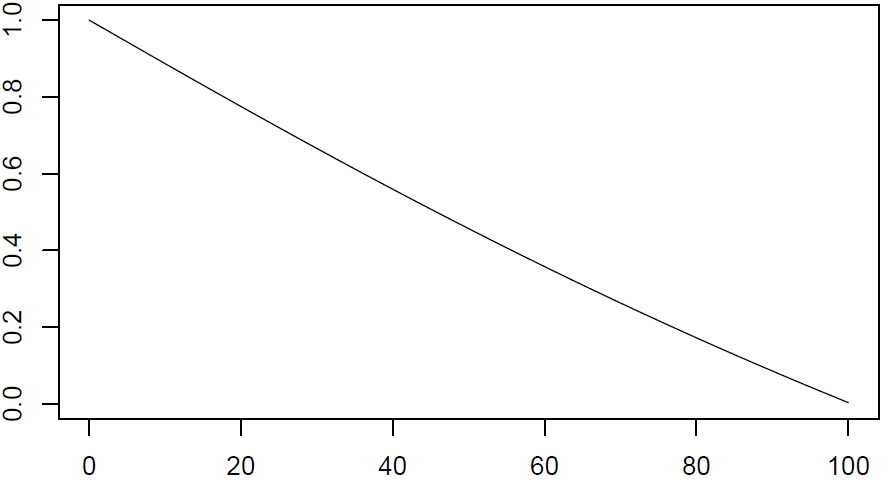
\includegraphics[width=0.9\textwidth]{img/Ajuste-alfa.png}
\end{center}

\caption{Linealidad de la figura \ref{fig2} ajustada.}
\label{fig5}
\end{figure}

\subsubsection{Resultados}

Utilizaremos para ver la influencia del valor $\alpha$ la siguiente figura:\\

\begin{figure}[H]
\begin{center}


\includegraphics[width=0.3\textwidth]{img/device3-1.png}
\end{center}

\caption{Cuadrado redondeado.}
\label{cuadrado-red}
\end{figure}

Podemos ver en la figura \ref{fig6}, que si tomamos un $\alpha$ asociado a un ángulo pequeño, en este ejemplo 45º, vemos que obtenemos unos resultados que varían de manera muy drástica.

\begin{figure}[H]
\begin{center}

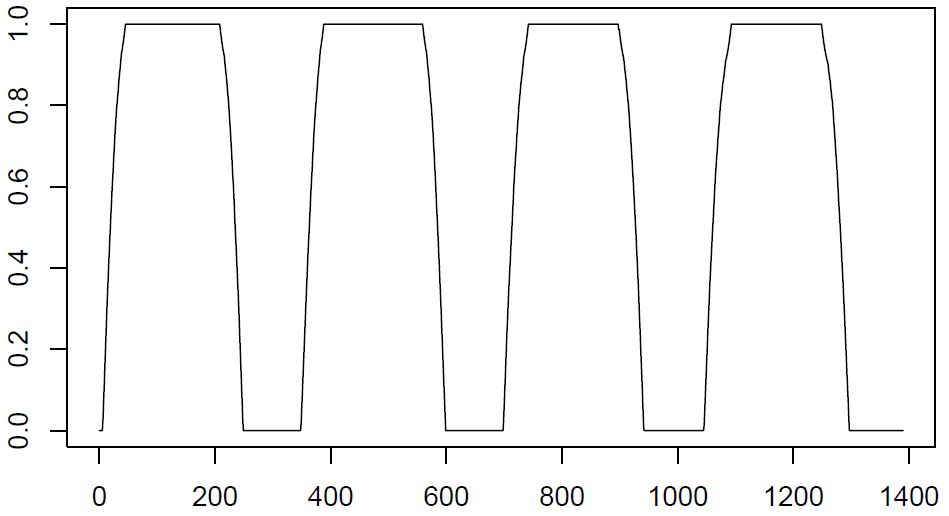
\includegraphics[width=0.9\textwidth]{img/lin-dev3-1-limpio-09075.png}
\end{center}

\caption{Linealidad del cuadrado redondeado con $\Theta = 45$ ($\alpha = 0.9075$).}
\label{fig6}
\end{figure}

De modo similar, en la figura \ref{fig7} podemos ver que si el ángulo seleccionado es demasiado permisivo, en el ejemplo 180º, se obtienen valores que nunca alcanzan el 0.\\

\begin{figure}[H]
\begin{center}

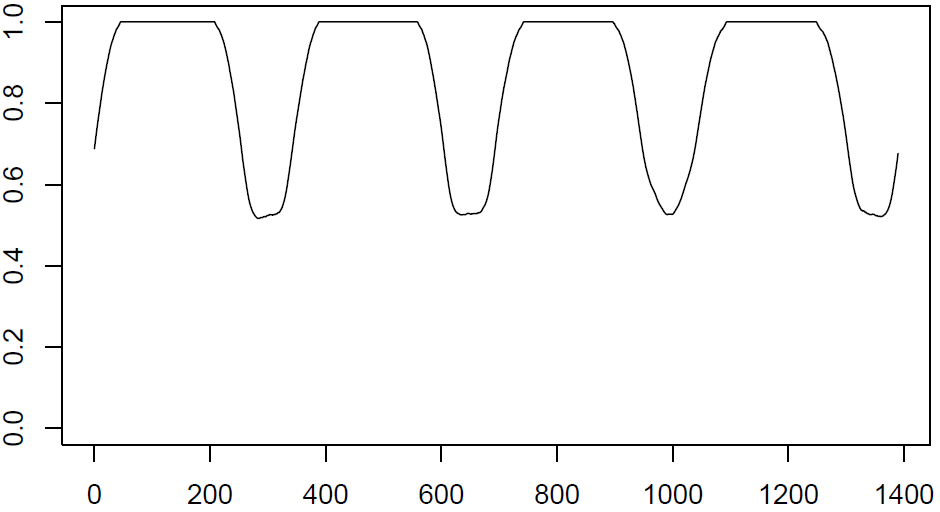
\includegraphics[width=0.9\textwidth]{img/lin-dev3-1-limpio-063.png}
\end{center}

\caption{Linealidad del cuadrado redondeado con $\Theta = 180$ ($\alpha = 0.63$).}
\label{fig7}
\end{figure}

En la figura \ref{fig8}, ajustando $\alpha$ a un valor intermedio, conseguimos un ajuste más apropiado para esta figura.\\

\begin{figure}[H]
\begin{center}

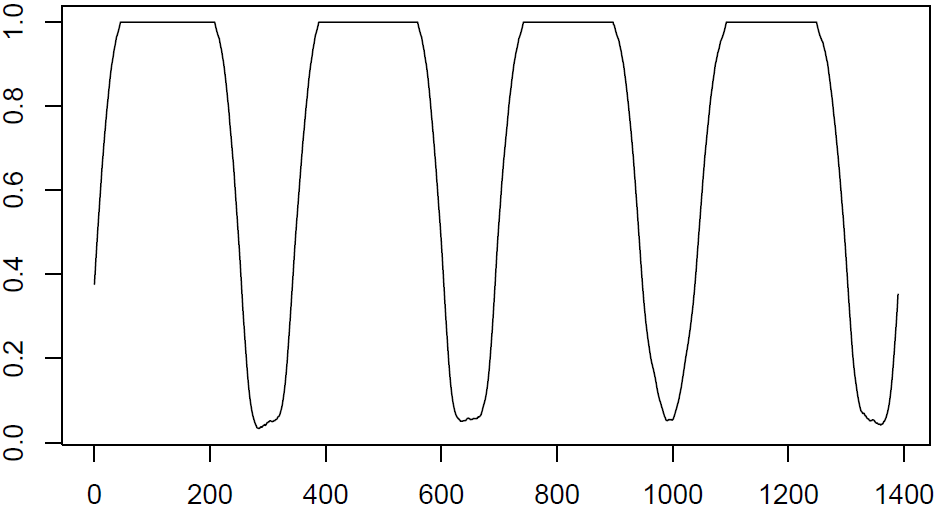
\includegraphics[width=0.9\textwidth]{img/lin-dev3-1-limpio-0815.png}
\end{center}

\caption{Linealidad del cuadrado redondeado con $\Theta = 90$ ($\alpha = 0.815$).}
\label{fig8}
\end{figure}

Se extrae por tanto que tenemos un buen comportamiento de esta primera propiedad, la linealidad, quedando libre el parámetro $\alpha$ para ser ajustado según las necesidades del problema a tratar, o dicho de otro modo, para poder ajustar lo que se considera que no es lineal.\\

\subsection{Curvacidad}


\subsubsection{Definición}

Entendemos la curvacidad como el grado en el que el segmento de un contorno es una curva. Se define como el opuesto de la linealidad, es decir:\\

\[
\ \tilde{U}(S^C_{ij}) = 1 - \tilde{L}^C_{ij}
\]
 
\subsubsection{Resultados}

Primero, veremos la gráfica de la curvacidad del cuadrado redondeado de la figura \ref{cuadrado-red}.

\begin{figure}[H]
\begin{center}
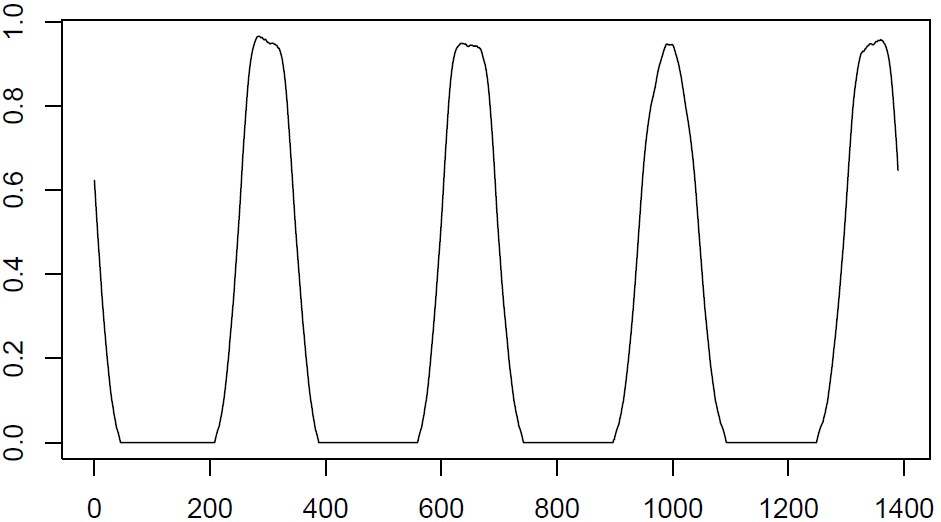
\includegraphics[width=0.9\textwidth]{img/nolin-dev3-1-limpio-0815.png}
\end{center}

\caption{Curvacidad de la imagen cuadrado redondeado.}
\label{fig9}
\end{figure}

Podemos ver en la figura \ref{fig9} que actúa como esperábamos, obteniendo 4 valores altos, que corresponden a las 4 esquinas de la figura. Además nos lleva a pensar que se tienen que comportar de manera similar a la curvatura.\\

En la figura \ref{fig10} podemos ver la gráfica de la curvacidad de una forma natural. Podemos observar que el comportamiento es adecuado, lo que reafirma el buen comportamiento de nuestras propiedades.\\

Sin embargo, podemos ver que todos los picos asociados a los giros son positivos. Esto muestra la desventaja de este modelo con respecto a la curvatura, que sí nos indica el sentido del giro mediante el signo del valor.\\

\begin{figure}[H]
\begin{center}

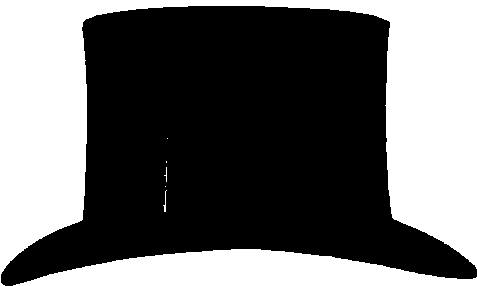
\includegraphics[width=0.3\textwidth]{img/hat-7.png} \hfill 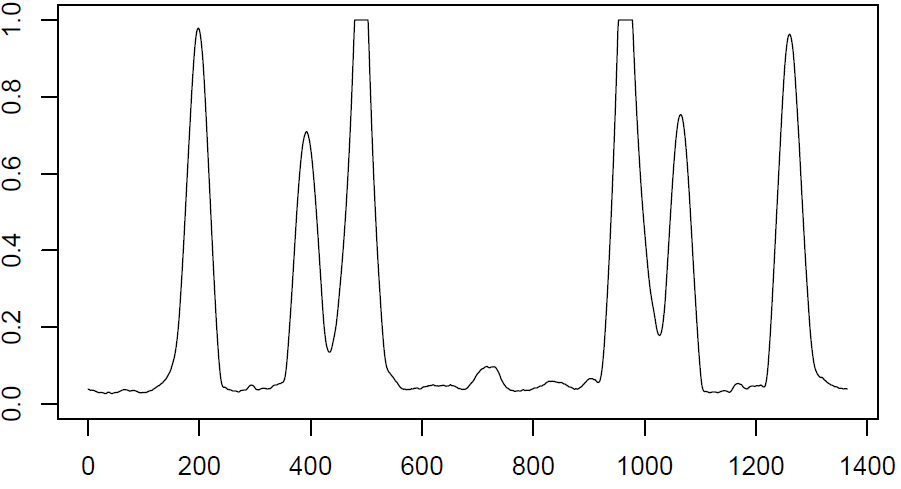
\includegraphics[width=0.6\textwidth]{img/nolin-hat-7.png}
\end{center}

\caption{Curvacidad de la imagen sombrero.}
\label{fig10}
\end{figure}


Evidentemente, al ser la propiedad opuesta a la linealidad, tiene la misma dependencia del parámetro $\alpha$, permitiendo ajustar que se considera curva según las necesidades del problema.\\

\subsection{Verticidad}

\subsubsection{Definición}
La verticidad describe el grado en el que un punto del contorno es un vértice.\\

En un vértice, se cumplen los siguiente hechos:
\begin{itemize}
\item Es el punto donde dos rectas se cortan, por tanto se espera una alta linealidad a izquierda y derecha del punto.
\item Las líneas que se cruzan en el vértice forman un ángulo, luego la linealidad en el punto se espera que sea baja. O dicho en otras palabras, que la curvacidad sea alta.
\end{itemize}

Por tanto, utilizando los conceptos creados anteriormente, se modela la verticidad como:\\

\[
\ \tilde{V}(C,i) = \otimes \left(\tilde{L}^C_{i-w,i}, \tilde{L}^C_{i,i+w},  \tilde{U}(S^C_{i-w/2,i+w/2})   \right)
\]
Con i el indice del punto en el contorno, $ \otimes $ una t-norma y $w$ el tamaño considerado de segmento. Se pueden añadir modificadores lingüísticos del tipo "muy" para enfatizar el cumplimiento de alguna de las características.

\subsubsection{Resultados}

Primero, veamos su comportamiento con una forma que contiene varios vértices reales y un vértice redondeado.\\

\begin{figure}[H]
\begin{center}


\includegraphics[width=0.3\textwidth]{img/fig4.png} \hfill 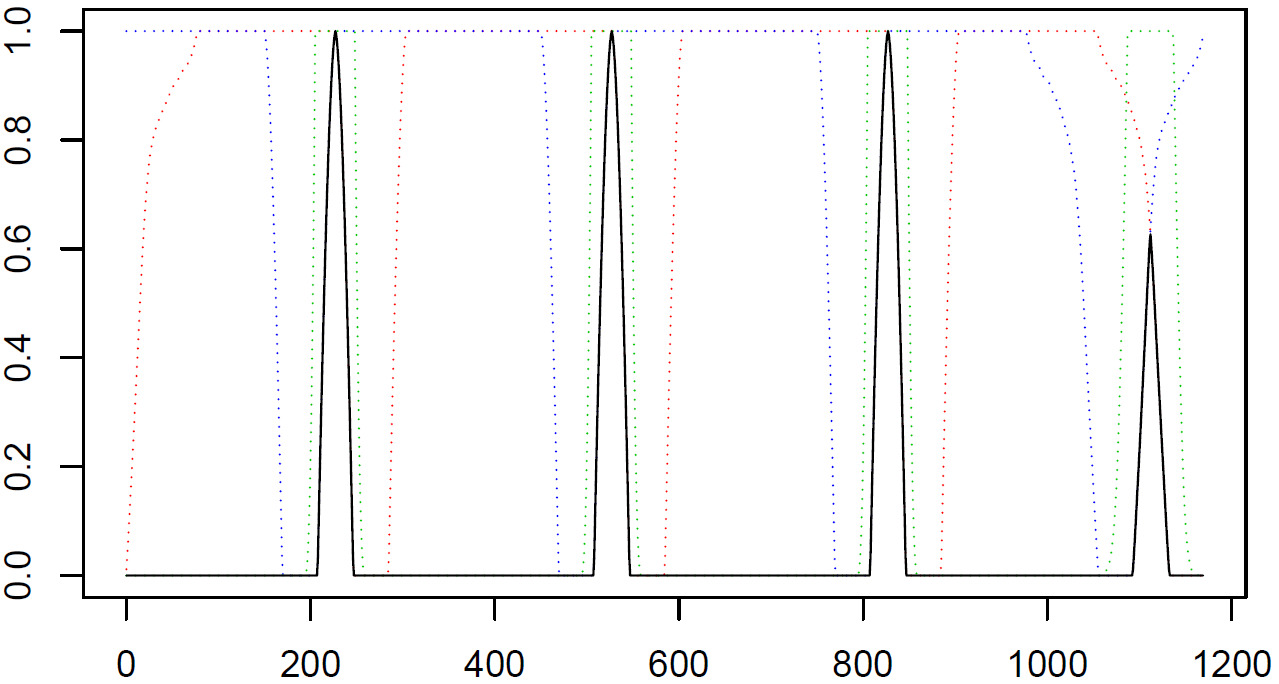
\includegraphics[width=0.6\textwidth]{img/vert-fig04-novvery.png}
\end{center}

\caption{Verticidad cuadrado con una esquina redondeada.}
\label{fig11}
\end{figure}

En la figura \ref{fig11} podemos ver que, efectivamente, nuestro grado de verticidad llega a 1 en los 3 vértices reales que tiene la figura y da un valor menor al vértice redondeado.\\

En la figura \ref{fig12} tenemos la verticidad del cuadrado redondeado. Al tener unas esquinas más redondeadas que en el caso de la figura \ref{fig11}, los valores que obtenemos son mucho menores, como es de esperar.\\

\begin{figure}[H]
\begin{center}


\includegraphics[width=0.3\textwidth]{img/device3-1.png} \hfill 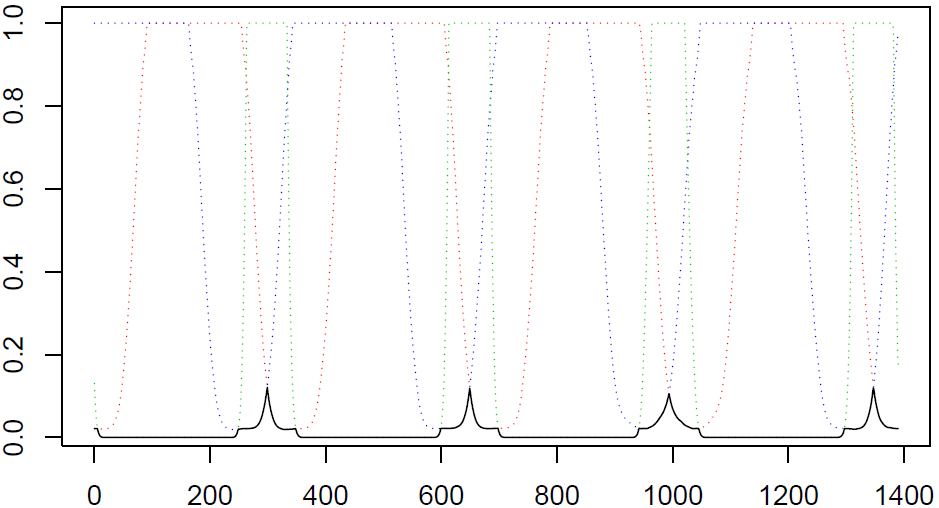
\includegraphics[width=0.6\textwidth]{img/vert-dev3-1-limpio.png}
\end{center}

\caption{Verticidad cuadrado redondeado.}
\label{fig12}
\end{figure}

Por tanto, la verticidad tiene un comportamiento deseable. Destacar que esta propiedad ha sido construida mediante el uso de propiedades más sencillas, intentando siempre utilizar los conceptos difusos para razonar.\\
